\documentclass{standalone}
\usepackage{tikz}
\usepackage{ctex,siunitx}
\usepackage{tkz-euclide}
\usepackage{amsmath}
\usetikzlibrary{patterns, calc}
\usetikzlibrary {decorations.pathmorphing, decorations.pathreplacing, decorations.shapes,}
\begin{document}
\small
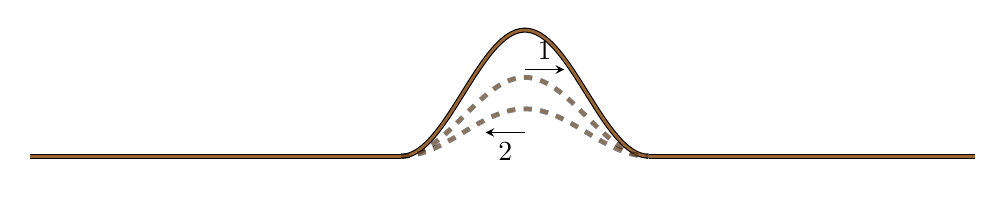
\begin{tikzpicture}[>=stealth, scale=1.0,samples=200]
  % \useasboundingbox(0,-0.6)rectangle(12,1.0);
  \draw [double=brown!80!black,double distance=1pt, domain=0:1.5*pi]  plot (\x,-0.5);
  \draw [double=brown!80!black,double distance=1pt, domain=1.5*pi:2.5*pi,dashed,opacity=0.5]  plot (\x,{0.5*cos(2*\x r)});
  \draw [double=brown!80!black,double distance=1pt, domain=1.5*pi:2.5*pi]  plot (\x,{0.5*cos(2*\x r)+0.3*cos(2*\x r)+0.3});
  \draw [double=brown!80!black,double distance=1pt, domain=1.5*pi:2.5*pi,dashed,opacity=0.5]  plot (\x,{0.3*cos(2*\x r)-0.2});
  \draw [double=brown!80!black,double distance=1pt, domain=2.5*pi:12]  plot (\x,-0.5);
  \draw[thin,->](2.0*pi,0.6)--++(0.5,0)node[above,midway]{1};
  \draw[thin,->](2.0*pi,-0.2)--++(-0.5,0)node[below,midway]{2};
\end{tikzpicture}
\end{document}